

{\setbeamercolor{background canvas}{bg=black}
	\begin{frame}[plain]
	\vfill
	\begin{columns}
		\column{.5\textwidth}
		\color{tumwhite}
		
		\Huge
		\visible<2->{\color{tumgray} Self-}{\color{white}Attention} \visible<2->{in \\ Deep Learning}
		
		\column{.5\textwidth}
		
		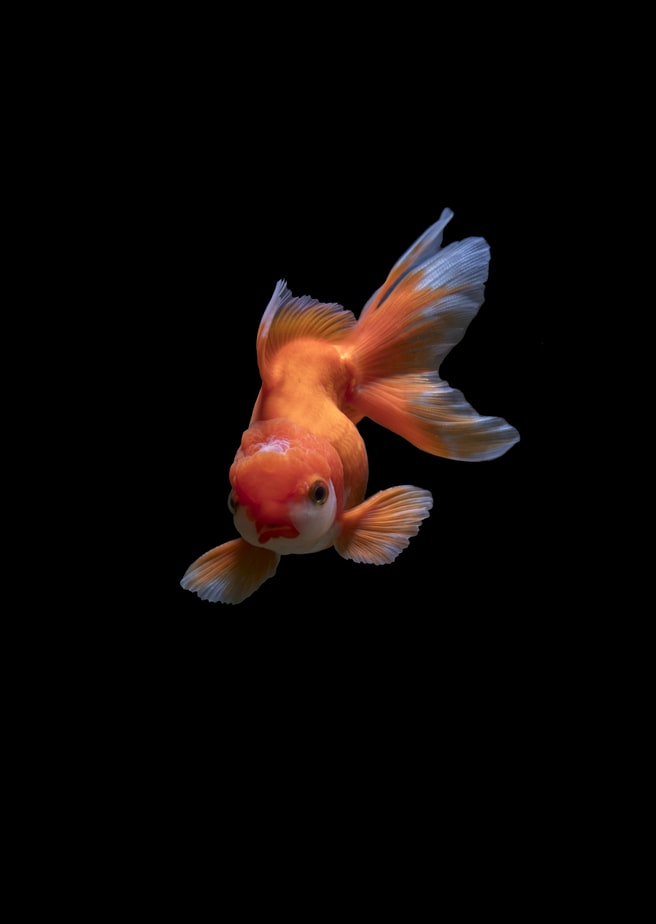
\includegraphics[width=6cm]{images/goldfish_zhengtaoTang}
	\end{columns}
	\begin{center}
		\Huge\color{tumwhite}
		\vfill\raggedleft
		{\small \color{tumgray} Photo by zhengtao tang on Unsplash}
		
	\end{center}
	\vfill
\end{frame}
}



\begin{frame}
	\only<1-4>{\frametitle{Attention}}
	\only<5>{\frametitle{Self-Attention}}
	
	\colorlet{querycolor}{tumorange}
	\colorlet{attentioncolor}{tumred}
	\colorlet{valuecolor}{tumblue}
	\colorlet{attentionoutcolor}{tumbluedark}
	\colorlet{keycolor}{tumgreen}
	
	\begin{columns}
		\column{.5\textwidth}
		
		\only<1>{
			\begin{itemize}[leftmargin=0em]
				\item Given a \textbf{sequence of observations}.
				\item We want to \textbf{calculate an output} based only on \textbf{classification-relevant} observations.
				\item This is realized by an weighted sum \\
				over \textbf{\color{tumbluedark}attention scores}
			\end{itemize}
			
			
		}
		\visible<2->{
\newcommand{\attnquery}{%
	\only<3>{%
		\begin{tikzpicture}[scale=0.6]
		\node[draw=querycolor, circle, fill=querycolor, fill opacity=.2, text opacity=1, font=\small, inner sep=.2em](a) at (0, 0){.2};
		\node[draw=querycolor, circle, fill=querycolor, fill opacity=.1, text opacity=1, font=\small, inner sep=.2em](b) at (1, 0){.1};
		\end{tikzpicture}
	}%
	\only<4->{%
		\begin{tikzpicture}[scale=0.4]
		\node[draw=querycolor, circle, fill=querycolor, fill opacity=.2, text opacity=1, font=\small, inner sep=.2em](a) at (0, 0){};
		\node[draw=querycolor, circle, fill=querycolor, fill opacity=.2, text opacity=1, font=\small, inner sep=.2em](a) at (0, 1){};
		\node[draw=querycolor, circle, fill=querycolor, fill opacity=.2, text opacity=1, font=\small, inner sep=.2em](a) at (0, 2){};
		\node[draw=querycolor, circle, fill=querycolor, fill opacity=.2, text opacity=1, font=\small, inner sep=.2em](a) at (0, 3){};
		
		\node[draw=querycolor, circle, fill=querycolor, fill opacity=.1, text opacity=1, font=\small, inner sep=.2em](b) at (1, 0){};
		\node[draw=querycolor, circle, fill=querycolor, fill opacity=.1, text opacity=1, font=\small, inner sep=.2em](b) at (1, 1){};
		\node[draw=querycolor, circle, fill=querycolor, fill opacity=.1, text opacity=1, font=\small, inner sep=.2em](b) at (1, 2){};
		\node[draw=querycolor, circle, fill=querycolor, fill opacity=.1, text opacity=1, font=\small, inner sep=.2em](b) at (1, 3){};
		
		\node[draw=querycolor, circle, fill=querycolor, fill opacity=.1, text opacity=1, font=\small, inner sep=.2em](b) at (2, 0){};
		\node[draw=querycolor, circle, fill=querycolor, fill opacity=.1, text opacity=1, font=\small, inner sep=.2em](b) at (2, 1){};
		\node[draw=querycolor, circle, fill=querycolor, fill opacity=.1, text opacity=1, font=\small, inner sep=.2em](b) at (2, 2){};
		\node[draw=querycolor, circle, fill=querycolor, fill opacity=.1, text opacity=1, font=\small, inner sep=.2em](b) at (2, 3){};
		
		\node[draw=querycolor, circle, fill=querycolor, fill opacity=.1, text opacity=1, font=\small, inner sep=.2em](b) at (3, 0){};
		\node[draw=querycolor, circle, fill=querycolor, fill opacity=.1, text opacity=1, font=\small, inner sep=.2em](b) at (3, 1){};
		\node[draw=querycolor, circle, fill=querycolor, fill opacity=.1, text opacity=1, font=\small, inner sep=.2em](b) at (3, 2){};
		\node[draw=querycolor, circle, fill=querycolor, fill opacity=.1, text opacity=1, font=\small, inner sep=.2em](b) at (3, 3){};
		\end{tikzpicture}
	}%
}


\newcommand{\attention}{%
	\only<2>{%
		\begin{tikzpicture}[scale=0.6]
		\node[draw=attentioncolor, circle, fill=attentioncolor, fill opacity=.4, text opacity=1, font=\small, inner sep=.2em](a) at (1,0){.2};
		\node[draw=attentioncolor, circle, fill=attentioncolor, fill opacity=.8, text opacity=1, font=\small, inner sep=.2em](b) at (2,0){.4};
		\node[draw=attentioncolor, circle, fill=attentioncolor, fill opacity=.2, text opacity=1, font=\small, inner sep=.2em](c) at (3,0){.1};
		\node[draw=attentioncolor, circle, fill=attentioncolor, fill opacity=.6, text opacity=1, font=\small, inner sep=.2em](d) at (4,0){.3};
		\end{tikzpicture}
	}%
	\only<3->{%
		\begin{tikzpicture}[scale=0.4]
		\node[draw=attentioncolor, circle, fill=attentioncolor, fill opacity=.4, text opacity=1, font=\small, inner sep=.2em](a) at (1,0){};
		\node[draw=attentioncolor, circle, fill=attentioncolor, fill opacity=.8, text opacity=1, font=\small, inner sep=.2em](b) at (2,0){};
		\node[draw=attentioncolor, circle, fill=attentioncolor, fill opacity=.2, text opacity=1, font=\small, inner sep=.2em](c) at (3,0){};
		\node[draw=attentioncolor, circle, fill=attentioncolor, fill opacity=.6, text opacity=1, font=\small, inner sep=.2em](d) at (4,0){};
		
		\node[draw=attentioncolor, circle, fill=attentioncolor, fill opacity=.4, text opacity=1, font=\small, inner sep=.2em](a) at (1,1){};
		\node[draw=attentioncolor, circle, fill=attentioncolor, fill opacity=.8, text opacity=1, font=\small, inner sep=.2em](b) at (2,1){};
		\node[draw=attentioncolor, circle, fill=attentioncolor, fill opacity=.2, text opacity=1, font=\small, inner sep=.2em](c) at (3,1){};
		\node[draw=attentioncolor, circle, fill=attentioncolor, fill opacity=.6, text opacity=1, font=\small, inner sep=.2em](d) at (4,1){};
		
		\node[draw=attentioncolor, circle, fill=attentioncolor, fill opacity=.4, text opacity=1, font=\small, inner sep=.2em](a) at (1,2){};
		\node[draw=attentioncolor, circle, fill=attentioncolor, fill opacity=.8, text opacity=1, font=\small, inner sep=.2em](b) at (2,2){};
		\node[draw=attentioncolor, circle, fill=attentioncolor, fill opacity=.2, text opacity=1, font=\small, inner sep=.2em](c) at (3,2){};
		\node[draw=attentioncolor, circle, fill=attentioncolor, fill opacity=.6, text opacity=1, font=\small, inner sep=.2em](d) at (4,2){};
		
		\node[draw=attentioncolor, circle, fill=attentioncolor, fill opacity=.4, text opacity=1, font=\small, inner sep=.2em](a) at (1,3){};
		\node[draw=attentioncolor, circle, fill=attentioncolor, fill opacity=.8, text opacity=1, font=\small, inner sep=.2em](b) at (2,3){};
		\node[draw=attentioncolor, circle, fill=attentioncolor, fill opacity=.2, text opacity=1, font=\small, inner sep=.2em](c) at (3,3){};
		\node[draw=attentioncolor, circle, fill=attentioncolor, fill opacity=.6, text opacity=1, font=\small, inner sep=.2em](d) at (4,3){};
		\end{tikzpicture}
	}%
}

\newcommand{\attnv}{%
	\only<2>{%
		\begin{tikzpicture}[scale=0.6]
		\node[draw=valuecolor, circle, fill=valuecolor, fill opacity=.2, text opacity=1, font=\small, inner sep=.2em](a) at (0, 1){.2};
		\node[draw=valuecolor, circle, fill=valuecolor, fill opacity=.1, text opacity=1, font=\small, inner sep=.2em](b) at (0, 2){.1};
		\node[draw=valuecolor, circle, fill=valuecolor, fill opacity=.3, text opacity=1, font=\small, inner sep=.2em](c) at (0, 3){.3};
		\node[draw=valuecolor, circle, fill=valuecolor, fill opacity=.4, text opacity=1, font=\small, inner sep=.2em](d) at (0, 4){.4};
		\end{tikzpicture}
	}%
	\only<3->{%
		\begin{tikzpicture}[scale=0.4]
		\node[draw=valuecolor, circle, fill=valuecolor, fill opacity=.2, text opacity=1, font=\small, inner sep=.2em](a) at (0, 1){};
		\node[draw=valuecolor, circle, fill=valuecolor, fill opacity=.1, text opacity=1, font=\small, inner sep=.2em](b) at (0, 2){};
		\node[draw=valuecolor, circle, fill=valuecolor, fill opacity=.3, text opacity=1, font=\small, inner sep=.2em](c) at (0, 3){};
		\node[draw=valuecolor, circle, fill=valuecolor, fill opacity=.4, text opacity=1, font=\small, inner sep=.2em](d) at (0, 4){};
		
		\node[draw=valuecolor, circle, fill=valuecolor, fill opacity=.2, text opacity=1, font=\small, inner sep=.2em](a) at (1, 1){};
		\node[draw=valuecolor, circle, fill=valuecolor, fill opacity=.1, text opacity=1, font=\small, inner sep=.2em](b) at (1, 2){};
		\node[draw=valuecolor, circle, fill=valuecolor, fill opacity=.3, text opacity=1, font=\small, inner sep=.2em](c) at (1, 3){};
		\node[draw=valuecolor, circle, fill=valuecolor, fill opacity=.4, text opacity=1, font=\small, inner sep=.2em](d) at (1, 4){};
		\end{tikzpicture}
	}%
}

\newcommand{\attnout}{%
	\only<2>{%
		\begin{tikzpicture}[scale=0.6]
		\node[draw=tumblack, circle, fill=attentionoutcolor, text=white, text opacity=1, font=\small, inner sep=.2em](d) at (0,0){.27};
		\end{tikzpicture}
	}	
	\only<3->{%
		\begin{tikzpicture}[scale=0.4]
		\node[draw=tumblack, circle, fill=attentionoutcolor, text=white, text opacity=1, font=\small, inner sep=.2em](d) at (0,0){};
		\node[draw=tumblack, circle, fill=attentionoutcolor, text=white, text opacity=1, font=\small, inner sep=.2em](d) at (0,1){};
		\node[draw=tumblack, circle, fill=attentionoutcolor, text=white, text opacity=1, font=\small, inner sep=.2em](d) at (0,2){};
		\node[draw=tumblack, circle, fill=attentionoutcolor, text=white, text opacity=1, font=\small, inner sep=.2em](d) at (0,3){};
		
		\node[draw=tumblack, circle, fill=attentionoutcolor, text=white, text opacity=1, font=\small, inner sep=.2em](d) at (1,0){};
		\node[draw=tumblack, circle, fill=attentionoutcolor, text=white, text opacity=1, font=\small, inner sep=.2em](d) at (1,1){};
		\node[draw=tumblack, circle, fill=attentionoutcolor, text=white, text opacity=1, font=\small, inner sep=.2em](d) at (1,2){};
		\node[draw=tumblack, circle, fill=attentionoutcolor, text=white, text opacity=1, font=\small, inner sep=.2em](d) at (1,3){};
		\end{tikzpicture}
	}%
}

\newcommand{\attnkey}{
	\only<0>{%
		\begin{tikzpicture}[scale=0.6]
		\node[draw=keycolor, circle, fill=keycolor, fill opacity=.2, text opacity=1, font=\small, inner sep=.2em](a) at (0, 0){.2};
		\node[draw=keycolor, circle, fill=keycolor, fill opacity=.1, text opacity=1, font=\small, inner sep=.2em](b) at (1, 0){.1};
		\node[draw=keycolor, circle, fill=keycolor, fill opacity=.3, text opacity=1, font=\small, inner sep=.2em](c) at (2, 0){.3};
		\node[draw=keycolor, circle, fill=keycolor, fill opacity=.4, text opacity=1, font=\small, inner sep=.2em](d) at (3, 0){.4};
		
		\node[draw=keycolor, circle, fill=keycolor, fill opacity=.2, text opacity=1, font=\small, inner sep=.2em](a) at (0, 1){.2};
		\node[draw=keycolor, circle, fill=keycolor, fill opacity=.1, text opacity=1, font=\small, inner sep=.2em](b) at (1, 1){.1};
		\node[draw=keycolor, circle, fill=keycolor, fill opacity=.3, text opacity=1, font=\small, inner sep=.2em](c) at (2, 1){.3};
		\node[draw=keycolor, circle, fill=keycolor, fill opacity=.4, text opacity=1, font=\small, inner sep=.2em](d) at (3, 1){.4};
		\end{tikzpicture}
	}
	\only<4->{%
		\begin{tikzpicture}[scale=0.4]
		\node[draw=keycolor, circle, fill=keycolor, fill opacity=.2, text opacity=1, font=\small, inner sep=.2em](a) at (0, 0){};
		\node[draw=keycolor, circle, fill=keycolor, fill opacity=.1, text opacity=1, font=\small, inner sep=.2em](b) at (1, 0){};
		\node[draw=keycolor, circle, fill=keycolor, fill opacity=.3, text opacity=1, font=\small, inner sep=.2em](c) at (2, 0){};
		\node[draw=keycolor, circle, fill=keycolor, fill opacity=.4, text opacity=1, font=\small, inner sep=.2em](d) at (3, 0){};
		
		\node[draw=keycolor, circle, fill=keycolor, fill opacity=.2, text opacity=1, font=\small, inner sep=.2em](a) at (0, 1){};
		\node[draw=keycolor, circle, fill=keycolor, fill opacity=.1, text opacity=1, font=\small, inner sep=.2em](b) at (1, 1){};
		\node[draw=keycolor, circle, fill=keycolor, fill opacity=.3, text opacity=1, font=\small, inner sep=.2em](c) at (2, 1){};
		\node[draw=keycolor, circle, fill=keycolor, fill opacity=.4, text opacity=1, font=\small, inner sep=.2em](d) at (3, 1){};
		
		\node[draw=keycolor, circle, fill=keycolor, fill opacity=.2, text opacity=1, font=\small, inner sep=.2em](a) at (0, 2){};
		\node[draw=keycolor, circle, fill=keycolor, fill opacity=.1, text opacity=1, font=\small, inner sep=.2em](b) at (1, 2){};
		\node[draw=keycolor, circle, fill=keycolor, fill opacity=.3, text opacity=1, font=\small, inner sep=.2em](c) at (2, 2){};
		\node[draw=keycolor, circle, fill=keycolor, fill opacity=.4, text opacity=1, font=\small, inner sep=.2em](d) at (3, 2){};
		
		\node[draw=keycolor, circle, fill=keycolor, fill opacity=.2, text opacity=1, font=\small, inner sep=.2em](a) at (0, 3){};
		\node[draw=keycolor, circle, fill=keycolor, fill opacity=.1, text opacity=1, font=\small, inner sep=.2em](b) at (1, 3){};
		\node[draw=keycolor, circle, fill=keycolor, fill opacity=.3, text opacity=1, font=\small, inner sep=.2em](c) at (2, 3){};
		\node[draw=keycolor, circle, fill=keycolor, fill opacity=.4, text opacity=1, font=\small, inner sep=.2em](d) at (3, 3){};
		\end{tikzpicture}
	}%
}

\begin{tikzpicture}[node distance=.2em]
\visible<2->{
\node[label={below:${\only<2>{\V{\alpha}\T}\only<3->{\M{A}\T}}$}, draw=attentioncolor, rounded corners](alpha){\attention};
\node[right=of alpha, label={right:${\only<2>{h}\only<3-4>{\M{H}}}$}](out){\attnout};
\node[above=of out, label={above:${\only<2>{\V{v}}\only<3-4>{\M{V}}}$}, draw=valuecolor, rounded corners](v){\attnv};
}
\visible<4->{
\node[above=of alpha, label={above:$\M{K}$}, draw=keycolor, rounded corners](k){\attnkey};
\node[left=of alpha, label={below:${\only<3>{\V{q}}\only<4->{\M{Q}}}\T$}, draw=querycolor, rounded corners](q){\attnquery};
}
\visible<5>{
\node[fill=white, text=black, fill opacity=0.5, text opacity=1, rounded corners] at (v){$\M{X}\Mweight_V$};
\node[fill=white, text=black, fill opacity=0.5, text opacity=1, rounded corners] at (k){$\M{X}\Mweight_K$};
\node[fill=white, text=black, fill opacity=0.5, text opacity=1, rounded corners] at (q){$\M{X}\Mweight_Q$};
}
\end{tikzpicture}}
		
		
		%	\begin{equation*}
		%		\text{Attention}(Q,K,V) = 
		%		\begin{tikzpicture}
		%		\node(alpha){$\underbrace{\attention}_\alpha$};
		%		\node[right=of alpha](out){};
		%		\node[above=of out]{\attnv};
		%		\end{tikzpicture}
		%		 
		%	\end{equation*}
		
		
		\column{.5\textwidth}
		
		\begin{tikzpicture}[yscale=3]
			
			\visible<4->{
				\node[draw=valuecolor, circle, fill=valuecolor, fill opacity=.2, text opacity=1, font=\small, inner sep=.2em](d) at (1,.35){};
				\node[draw=valuecolor, circle, fill=valuecolor, fill opacity=.1, text opacity=1, font=\small, inner sep=.2em](e) at (2,.05){};
				\node[draw=valuecolor, circle, fill=valuecolor, fill opacity=.3, text opacity=1, font=\small, inner sep=.2em](f) at (3,.42){};
				\node[draw=valuecolor, circle, fill=valuecolor, fill opacity=.4, text opacity=1, font=\small, inner sep=.2em](g) at (4,.25){};
				\draw (d) -- (e) -- (f) -- (g);
			}
			
			\node[draw=valuecolor, circle, fill=valuecolor, fill opacity=.2, text opacity=1, font=\small, inner sep=.2em](a) at (1,.3){};
			\node[draw=valuecolor, circle, fill=valuecolor, fill opacity=.1, text opacity=1, font=\small, inner sep=.2em](b) at (2,.1){};
			\node[draw=valuecolor, circle, fill=valuecolor, fill opacity=.3, text opacity=1, font=\small, inner sep=.2em](c) at (3,.3){};
			\node[draw=valuecolor, circle, fill=valuecolor, fill opacity=.4, text opacity=1, font=\small, inner sep=.2em](d) at (4,.4){};
			
			\draw (a) -- (b) -- (c) -- (d);
			
			\foreach \t in {1,2,3,4} {
				\draw[tumgray] (\t,0) -- (\t,-.05) node[at end, below, text=tumgray] {$t_\t$};
			}
			
			%\draw[-stealth] (0,0) -- (0,.5);
			\draw[-stealth, tumgray] (.5,0) -- (4.5,0);
			
			\only<2,3>{
			\node[draw=tumblack, circle, fill=attentionoutcolor, text=white, fill opacity=1, text opacity=1, font=\small, inner sep=.2em, label={right:$\sum_{t=0}^{T} \alpha_t v_t = \V{\alpha}^T \V{v}$}](out) at (2.5,-.5) {};
			}
			\only<4->{
			\node[draw=white, circle, fill=attentionoutcolor, text=white, fill opacity=1, text opacity=1, font=\small, inner sep=.2em](outba) at (1.05,-.48) {};
			\node[draw=white, circle, fill=attentionoutcolor, text=white, fill opacity=1, text opacity=1, font=\small, inner sep=.2em](outbb) at (2.05,-.48) {};
			\node[draw=white, circle, fill=attentionoutcolor, text=white, fill opacity=1, text opacity=1, font=\small, inner sep=.2em](outbc) at (3.05,-.48) {};
			\node[draw=white, circle, fill=attentionoutcolor, text=white, fill opacity=1, text opacity=1, font=\small, inner sep=.2em](outbd) at (4.05,-.48) {};
				
			\node[draw=white, circle, fill=attentionoutcolor, text=white, fill opacity=1, text opacity=1, font=\small, inner sep=.2em](outa) at (1,-.5) {};
			\node[draw=white, circle, fill=attentionoutcolor, text=white, fill opacity=1, text opacity=1, font=\small, inner sep=.2em](out) at (2,-.5) {};
			\node[draw=white, circle, fill=attentionoutcolor, text=white, fill opacity=1, text opacity=1, font=\small, inner sep=.2em](outa) at (3,-.5) {};
			\node[draw=white, circle, fill=attentionoutcolor, text=white, fill opacity=1, text opacity=1, font=\small, inner sep=.2em](outa) at (4,-.5) {};

			}
		
			\node at (2.5, -.25) {};
			
			\visible<2->{
			\draw[-stealth, draw=tumred, opacity=.4, line width=.4] (a) -- (out);
			\draw[-stealth, draw=tumred, opacity=.8, line width=.8] (b) -- (out);
			\draw[-stealth, draw=tumred, opacity=.2, line width=.2] (c) -- (out);
			\draw[-stealth, draw=tumred, opacity=.6, line width=.6] (d) -- (out);
			}
			
			\visible<1>{
				\node(annot1) at (5.5,.1){relevant};
				\draw[-stealth, tumred, shorten <= .3em, , shorten >= .3em](annot1) -- (b);
				\draw[-stealth, tumred, shorten <= .3em, , shorten >= .3em](annot1) -- (d);
				
				\node(annot2) at (3.5,.85){not relevant};
				\draw[-stealth, tumbluelight, shorten <= 1em, shorten >= 1em](annot2) -- (a);
				\draw[-stealth, tumbluelight, shorten <= 1em, shorten >= 1em](annot2) -- (c);
			}
			
		\end{tikzpicture}
%		

	\end{columns}

	
	\Large
	\only<2>{
	\begin{equation*}
	\text{Attention}({\color{tumred}\V{\alpha}}, {\color{tumblue}\V{v}}) = {\color{tumred}\V{\alpha}}^T  {\color{tumblue}\V{v}} = \sum_{t=0}^{T} \alpha_tv_t, \quad \V{\alpha} \in [0,1]^{T=4}, \V{v} \in \mathbb{R}^{T}
	\end{equation*}
	}
	\only<3>{
		\begin{equation*}
		\text{Attention}({\color{tumorange}\V{K}}, {\color{tumgreen}\V{q}}, {\color{tumblue}\V{v}}) = 
		\overbrace{\text{softmax}\left({\color{tumgreen}\V{q}^T}{\color{tumorange}\V{K}}\right)}^{{\color{tumred}\V{\alpha}}^T}
		{\color{tumblue}\V{v}}, \quad \V{v} \in \mathbb{R}^{T}, \V{q} \in \mathbb{R}^{D_k}, \M{K} \in \mathbb{R}^{D_k \times T}
		\end{equation*}
	}
	\only<4>{
		\begin{equation*}
		\text{Attention}({\color{tumorange}\V{K}}, {\color{tumgreen}\V{Q}}, {\color{tumblue}\V{V}}) = 
		\text{softmax}\left({\color{tumgreen}\V{Q}^T}{\color{tumorange}\V{K}}\right)
		{\color{tumblue}\V{V}}, \quad \V{V} \in \mathbb{R}^{T \times D_v}, \V{Q}, \M{K} \in \mathbb{R}^{D_k \times T}, \M{\alpha} \in \mathbb{R}^{T \times T}
		\end{equation*}
	}
	\only<5>{
		\begin{equation*}
		\text{Self-Attention}_\Mweight(\M{X}) = \text{Attention}(\M{X}\Mweight_K, \M{X}\Mweight_Q, \M{X}\Mweight_V) = \text{softmax}\left(\left(\M{X}\Mweight_Q\right)\left(\M{X}\Mweight_K\right)\right)\left(\M{X}\Mweight_V\right)
		\end{equation*}
	}
\end{frame}

\begin{frame}
	\frametitle{Visualize the Attention Matrix as Adjacency Matrix}
	\centering\begin{tikzpicture}[inner sep=0]
		\node[inner sep=0](alpha){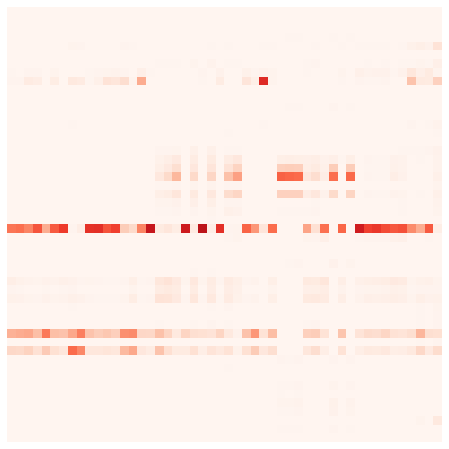
\includegraphics[width=6cm]{images/self-attention/transformer/self-attention-1/head0_imshow}};
		\node[left=0em of alpha]{$T_\text{in}$};
		\node[right=of alpha](colorbar){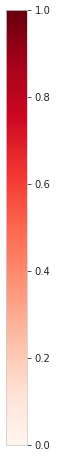
\includegraphics[height=6cm]{images/self-attention/colorbar}};
		\node[below=0em of alpha]{$T_\text{out}$};
	\end{tikzpicture}
\end{frame}

\begin{frame}

\frametitle{Visualize the Attention Matrix as Bipartite Graph}
	\begin{tikzpicture}
		\node[inner sep=0](alpha){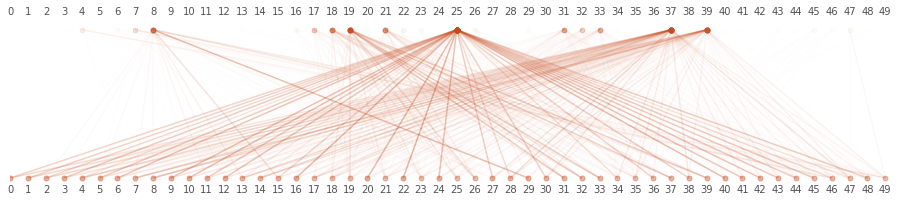
\includegraphics[width=\textwidth]{images/self-attention/transformer/self-attention-1/head0_conn}};
		\node[above=0em of alpha]{$T_\text{in}$};
		\node[below=0em of alpha]{$T_\text{out}$};
	\end{tikzpicture}
	
\end{frame}

\begin{frame}
	\frametitle{Attention Scores in Context of Input Time Series}
	\framesubtitle{Head 1}
	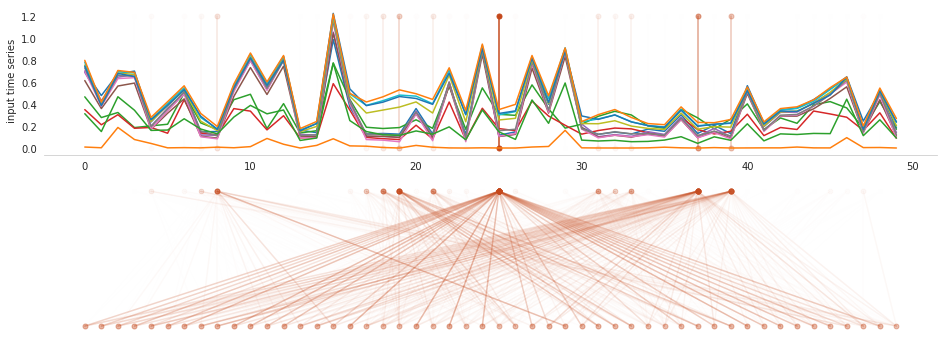
\includegraphics[width=\textwidth]{images/self-attention/transformer/self-attention-1/head0_conn_input}
\end{frame}

\begin{frame}
\frametitle{Attention Scores in Context of Input Time Series}
\framesubtitle{Head 2}
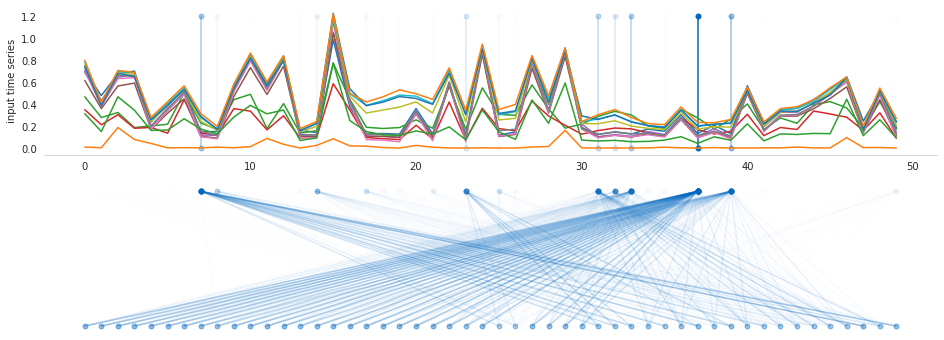
\includegraphics[width=\textwidth]{images/self-attention/transformer/self-attention-1/head1_conn_input}
\end{frame}

\begin{frame}
\frametitle{Attention Scores in Context of Input Time Series}
\framesubtitle{Head 3}
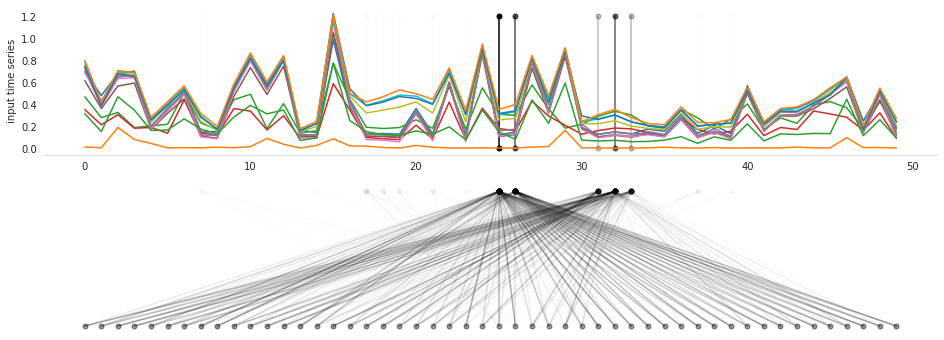
\includegraphics[width=\textwidth]{images/self-attention/transformer/self-attention-1/head2_conn_input}
\end{frame}

%\begin{frame}
%	\frametitle{Transformer}
%	
%	\tikzstyle{conn} = [-stealth, rounded corners, tumbluedark, thick]
%	\tikzstyle{module} = [draw=none, fill=tumgraylight, rounded corners]
%	\tikzstyle{layer} = [draw=none, fill=tumbluelight, rounded corners]
%	
%	\newcommand{\attentionblock}{
%	\begin{tikzpicture}[node distance=2em]
%%		\node(input){inputs};
%%		\node[below of=input](plus){+};
%%		\node[left of=plus](posenc){p};
%		
%		\node[module](attn){Multi-Head-Attention};
%		\node[module, below=.5em of attn](addnorm){Add \& Norm};
%		
%		\node[module, below=2em of addnorm](ff){Feed Forward};
%		\node[module, below=.5em of ff](addnorm2){Add \& Norm};
%		
%		
%		\coordinate[above=of attn](in);
%		\coordinate[below=of addnorm2](out);
%		\draw[conn] (in) -- (attn);
%		\draw[conn] (in) -- ($ (attn)!.5!(in) $) -| ($ (attn.north)+(2em,0) $);
%		\draw[conn] (in) -- ($ (attn)!.5!(in) $) -| ($ (attn.north)-(2em,0) $);  
%		%		
%		\draw[conn] (in) -- ($ (attn)!.6!(in) $) -| ($ (attn.east)+(.5em,0) $) |- (addnorm.east);
%		
%		\draw[conn] (attn) -- (addnorm);
%		
%		\draw[conn] (addnorm) -- (ff);
%		\draw[conn] (addnorm) -- ($ (addnorm)!.5!(ff) $) -| ($ (ff.east)+(.5em,0) $) |- (addnorm2.east);
%		\draw[conn] (ff) -- (addnorm2);
%		\draw[conn] (addnorm2) -- (out);
%		
%		\begin{pgfonlayer}{background}
%		\node[layer, draw=black, fit=(attn)(addnorm)(ff)(addnorm2)(in)(out)]{};
%		\end{pgfonlayer}
%		
%		\end{tikzpicture}
%		}
%	\begin{tikzpicture}
%		\node(input){input $\M{X}$};
%		\node[below=of input](posend){posenc};
%	\end{tikzpicture}
%	
%\end{frame}

\begin{frame}
\frametitle{Self-Attention Block 1}
\framesubtitle{Head 1}
\centering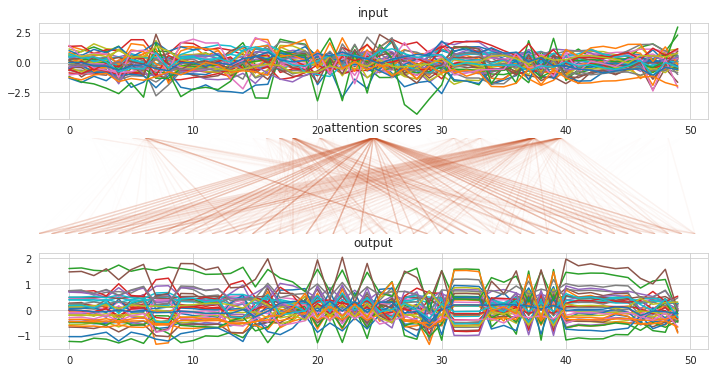
\includegraphics[width=.85\textwidth]{images/self-attention/transformer/self-attention-1}
\end{frame}


\begin{frame}
\frametitle{Self-Attention Block 2}
\framesubtitle{Head 1}
\centering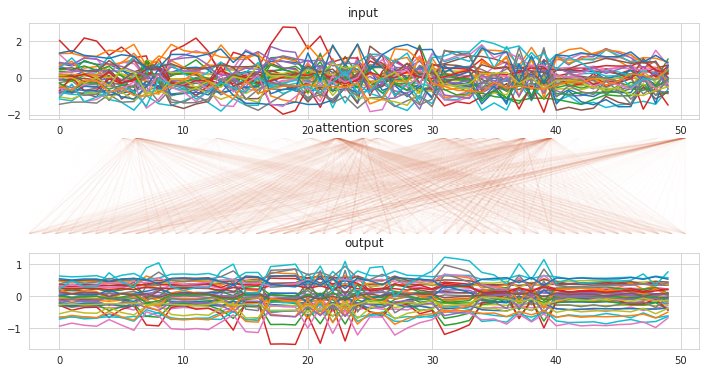
\includegraphics[width=.85\textwidth]{images/self-attention/transformer/self-attention-2}
\end{frame}


\begin{frame}
\frametitle{Self-Attention Block 3}
\framesubtitle{Head 1}
\centering
\begin{tikzpicture}
	\node(a){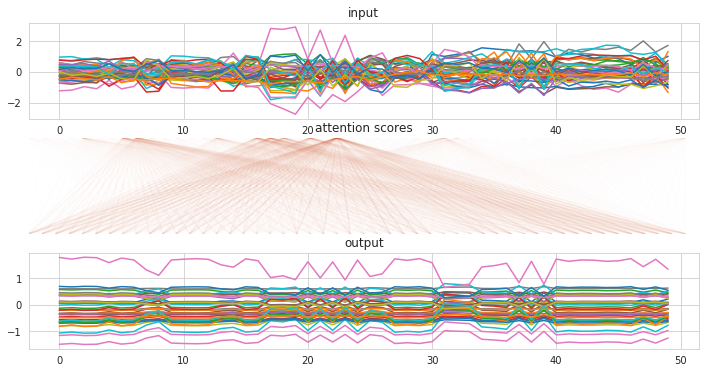
\includegraphics[width=.85\textwidth]{images/self-attention/transformer/self-attention-3}};
	\node[fill=tumbluedark, text=white, rounded corners, font=\Large, yshift=-2cm] at (a){maxpooling};
\end{tikzpicture}
\end{frame}

\begin{frame}
\frametitle{Classification Scores after Outlinear + Softmax}
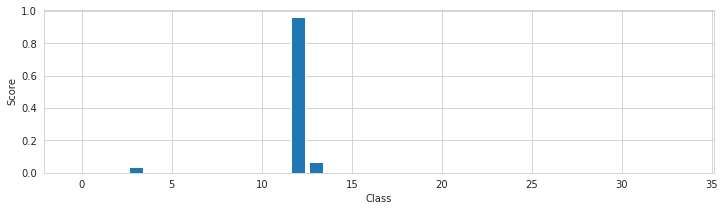
\includegraphics[width=.85\textwidth]{images/self-attention/transformer/outlinear}
\end{frame}
